

\chapter{Levitaci'on ac'ustica}
\section{Introducci'on}
\section{Antecedentes}
\section{N'umeros adimensionales}
\section{Refinamiento de malla}
Como en todos los m'etodos num'ericos, se debe realizar un refinamiento de malla
para encontrar la mejor relaci'on entre los resultados y el tiempo de computo
\section{Fuerza sobre un cilindro en una onda estacionaria}
\section{Levitaci'on en una cavidad con reflector plano}
\section{Levitaci'on en una cavidad con reflector redondo}
\section{Conclusiones}



\section{Teor'ia y aplicaciones}

Un objeto sumergido en un campo de sonido experimenta fuerzas asociadas a 
este campo. La magnitud de la fuerza es igual al promedio de la cantidad
de movimiento que atravieza una superficie  $A$. Esta fuerza es
muy debil para el caso de una onda viajera. En 1866, Kundt fue el
primero en medir la magnitud de estas fuerzas a trav'es del movimiento
de part'iculas de polvo en un tubo con un campo de sonido en resonancia~\cite{kundt1866}.
Fue hasta 1934, que L. V. King desarroll'o la teor'ia para medir la
fuerza incidente en un objeto sumergido en una onda viajera o una onda estacionaria,
y as'i poder explicar  los patrones de estrias formados en los experimentos
desarrollados por Kundt~\cite{king34}. King desarroll'o la teor'ia para el caso
de esferas r'igidas sumergidas en un fluido inviscido. Yosioka \etal extendieron
el trabajo de King para el caso de esferas compresibles o burbujas. El trabajo 
original de King no era suficiente para predecir las posiciones de equilibrio
de burbujas sumergidas en una onda plana estacionaria. En 1962, usando un enfoque
diferente, Gor'kov deriv'o un m'etodo muy simple para calcular la fuerza sobre una
part'icula en un campo de sonido cualquiera y demostrando que las soluciones eran
equivalentes para el caso de una onda de sonido estacionaria~\cite{gorkov62}.
Barmatz \etal desarrollaron una metodolog'ia para determinar la fuerza de levitaci'on
y la estabilidad de las esferas levitadas bajo diferentes geometr'ias~\cite{barmatz84}. 
Xie \etal toman del art'iculo de Gor'kov la formula para calcular el potencial ac'ustico
y la metodolog'ia desarrollada por Barmatz \etal, y optimizan la geometr'ia para maximizar
la fuerza, resolviendo el campo de velocidades mediante el m'etodo de elemento de frontera~\cite{xie}.

Un dispositivo levitador ac'ustico de un eje consta principalmente de tres partes,
el emisor o fuente de sonido, un reflector y el fluido en el cual el emisor y el
reflector estan inmersos, como se muestra en la figura~\ref{fig:device}. Esta figura
representa al modelo m'as sencillo de un dispositivo de levitaci'on ac'ustica de un eje. El
emisor oscila con frecuencia $\omega=2\pi/\lambda$ y amplitud $v_o$, donde $\lambda$ es la
longitud de onda. La onda de sonido viaja y se refleja en (b) y despu'es de un tiempo forma
una onda estacionaria a la cual se le asocia un potencial ac'ustico que puede ser capaz de levitar
part'iculas s'olidas, siempre y cuando el radio de la part'icula sea menor a la longitud de
onda del dispositivo.
 
\begin{figure}
\centering
\begin{pspicture}(3,4.35)
%\psgrid
%
\psframe(0,0)(3,1)
\psframe(0,4)(3,3)
\psline[linewidth=0.1mm,linestyle=dashed]{<->}(-.25,1)(-.25,3)
\psline[linewidth=0.1mm,linestyle=dashed]{<->}(0,4.25)(3,4.25)

\psline{<->}(0,.75)(0,1.25)
\psline{<->}(0.5,.75)(0.5,1.25)
\psline{<->}(1,.75)(1,1.25)
\psline{<->}(1.5,.75)(1.5,1.25)
\psline{<->}(2,.75)(2,1.25)
\psline{<->}(2.5,.75)(2.5,1.25)
\psline{<->}(3,.75)(3,1.25)
\rput[C](1.5,.5){(a)}
\rput[C](1.5,3.5){(b)}
\rput[C](2.5,2){(c)}
%
\rput[C](1.5,4.35){$w$}
\rput[C](-.4,2){$h$}
%

%
\end{pspicture}
\caption{\label{fig:device}
Esquema de un levitador ac'ustico de un eje. El dispositivo est'a formado por tres partes,
(a) la fuente de sonido que oscila con velocidad $v_o$, (b) el reflector y (c) el fluido
en el cual se forma la onda estacionaria y levitan las part'iculas. El dispositivo tiene
dimensiones $w$ de ancho y $h$ de altura.
}
\end{figure}

  
El potencial ac'ustico desarrollado por Gor'kov~\cite{gorkov62} es
\begin{equation}\label{eq:U}
U=2\pi r^3\left( \frac{\PROM{p_{in}^2}}{3\rho_f c_s^2}-\frac{\rho_f\PROM{v_{in}^2}}{2}\right)
\end{equation}
donde $r$ es el radio de la part'icula suspendida, $\PROM{p_{in}^2}$ y $\PROM{v_{in}}$ son las
fluctuaciones medias al cuadrado de la presi'on y la velocidad, respectivamente y $\rho_f$ y
$c_s$ son la densidad del fluido y la velocidad del sonido en el mismo. Para el caso de cero 
gravedad, las posiciones de levitacion corresponden a los m'inimos del potencial, donde 
se satisface $\partial U/\partial y=0$, donde $y$ representa la coordenada vertical. 
Los componentes de la fuerza alrededor del m'inimo
del potencial se caracterizan por ser una fuerza de restauraci'on, la cual empuja a la 
part'icula a la posici'on de equilibrio si una fuerza aleatoria o una perturbaci'on peque~na
actue sobre ella. La fuerza de restauraci'on se puede escribir como $F = -\kappa \Delta y$, donde
$\kappa$ es la constante de restauraci'on de la fuerza  y $\Delta y$ representa al desplazamiento
de la posici'on de equilibrio. La fuerza ac'ustica y la constante de restauraci'on de la fuerza
se pueden expresar en terminos del potencial ~(\ref{eq:U}) como 
\begin{equation}\label{eq:F}
F = -\frac{\partial U}{\partial y}
\end{equation}
y
\begin{equation}
\kappa = - \frac{\partial^2U}{\partial y^2},
\end{equation}
respectivamente.

Para el caso donde existe un campo gravitatorio, la posici'on de equilibrio en funci'on del potencial
se define ahora como,
\begin{equation}
F = -\frac{\partial U}{\partial y} = -m_p g,
\end{equation}
donde $m_p$ es la masa de la part'icula a levitar y $g$ el valor de la aceleraci'on debida a un campo gravitacional.

Para comparar las simulaciones numericas con los experimentos, es necesario definir los siguientes n'umeros
adimensionales, representados con un asterisco,
\begin{equation}
U^\ast = \frac{U}{2\pi r^3\rho_fv_o^2},
\end{equation}
para el potencial. La presi'on adimensional se define como
\begin{equation}
p^\ast = \frac{p}{rho_f c_s v_o}.
\end{equation}
La velocidad y las coordenadas horizontal y vertical se adimensionalizan como
\begin{equation}
u^\ast = \frac{u}{v_o},\qquad x^\ast = xk, \qquad y^\ast = yk,
\end{equation}
respectivamente. Por lo tanto la fuerza y la potencia adimensional se definen como
\begin{equation}
F^\ast = \frac{F}{2\pi r^3\rho_fv_o^2k}
\end{equation}
y
\begin{equation}
P^\ast  = \frac{Pk^2}{\rho_f c_s v_o^2},
\end{equation}
respectivamente.




\section{Levitaci'on en una cavidad con reflector plano}

Como se dijo en la secci'on anterior, el dispositivo de levitaci'on ac'ustica
m'as sencillo consta de un emisor que oscila con frecuencia angular $\omega=$,
y un reflector plano, como el que se mostr'o en la figura~\ref{fig:device}. Para
hacerlo m'as sencillo, se realizaron experimentos num'ericos en esta cavidad
con condiciones de frontera peri'odicas en la direcci'on horizontal.

Como primer paso, se determinan las frecuencias de resonancia para la cavidad.
Se sabe que para una cavidad cuadrada que contiene una onda plana, la resonancia
existe en
\begin{equation}
H_m=\frac{m\lambda}{2},
\end{equation}
donde $H_m$ es la altura de la cavidad y $m=1,\ldots,n$ corresponde al modo
de resonancia. En resonancia, la velocidad alcanza un m'aximo, por lo que 
monitoreando el valor de la velocidad m'axima se pueden localizar
experimentalmente las frecuencias de resonancia.

Para las simulaciones, se procedi'o de la siguiente manera; primero se defini'o
la altura de la cavidad y despu'es el modo al cual se quiere excitar
\begin{equation}\label{eq:modes}
\lambda = \frac{4h}{2m-1},
\end{equation}
donde $h$ es la altura de la cavidad y $m$ corresponde al modo de excitaci'on.

Las frecuencias de resonancia se pueden determinar experimentalmente, lo cual
es 'util para geometrias irregulares. Para hacerlo, se mide la potencia en la 
superficie del emisor $S_E$ como funci'on de la frecuencia
\begin{equation}
P = \int_{S_E}\PROM{p\cdot v_n}dS
\end{equation}
donde $\PROM{}$ se refiere al promedio temporal sobre un periodo, $v_n$ es la
velocidad normal a la superficie y $dS$ es el diferencial de la superficie. En la 
figura~\ref{fig:resonancia-cuadrada} se observa que los picos, correspondientes 
a frecuencias en resonancia, se encuentran en $h/\lambda=0.25,0.75,1.25,1.75$ y $2.25$
como se puede deducir de la ecuaci'on~\ref{eq:modes}.


\begin{figure}[h]
%GNUPLOT: LaTeX picture with Postscript
\begin{picture}(0,0)%
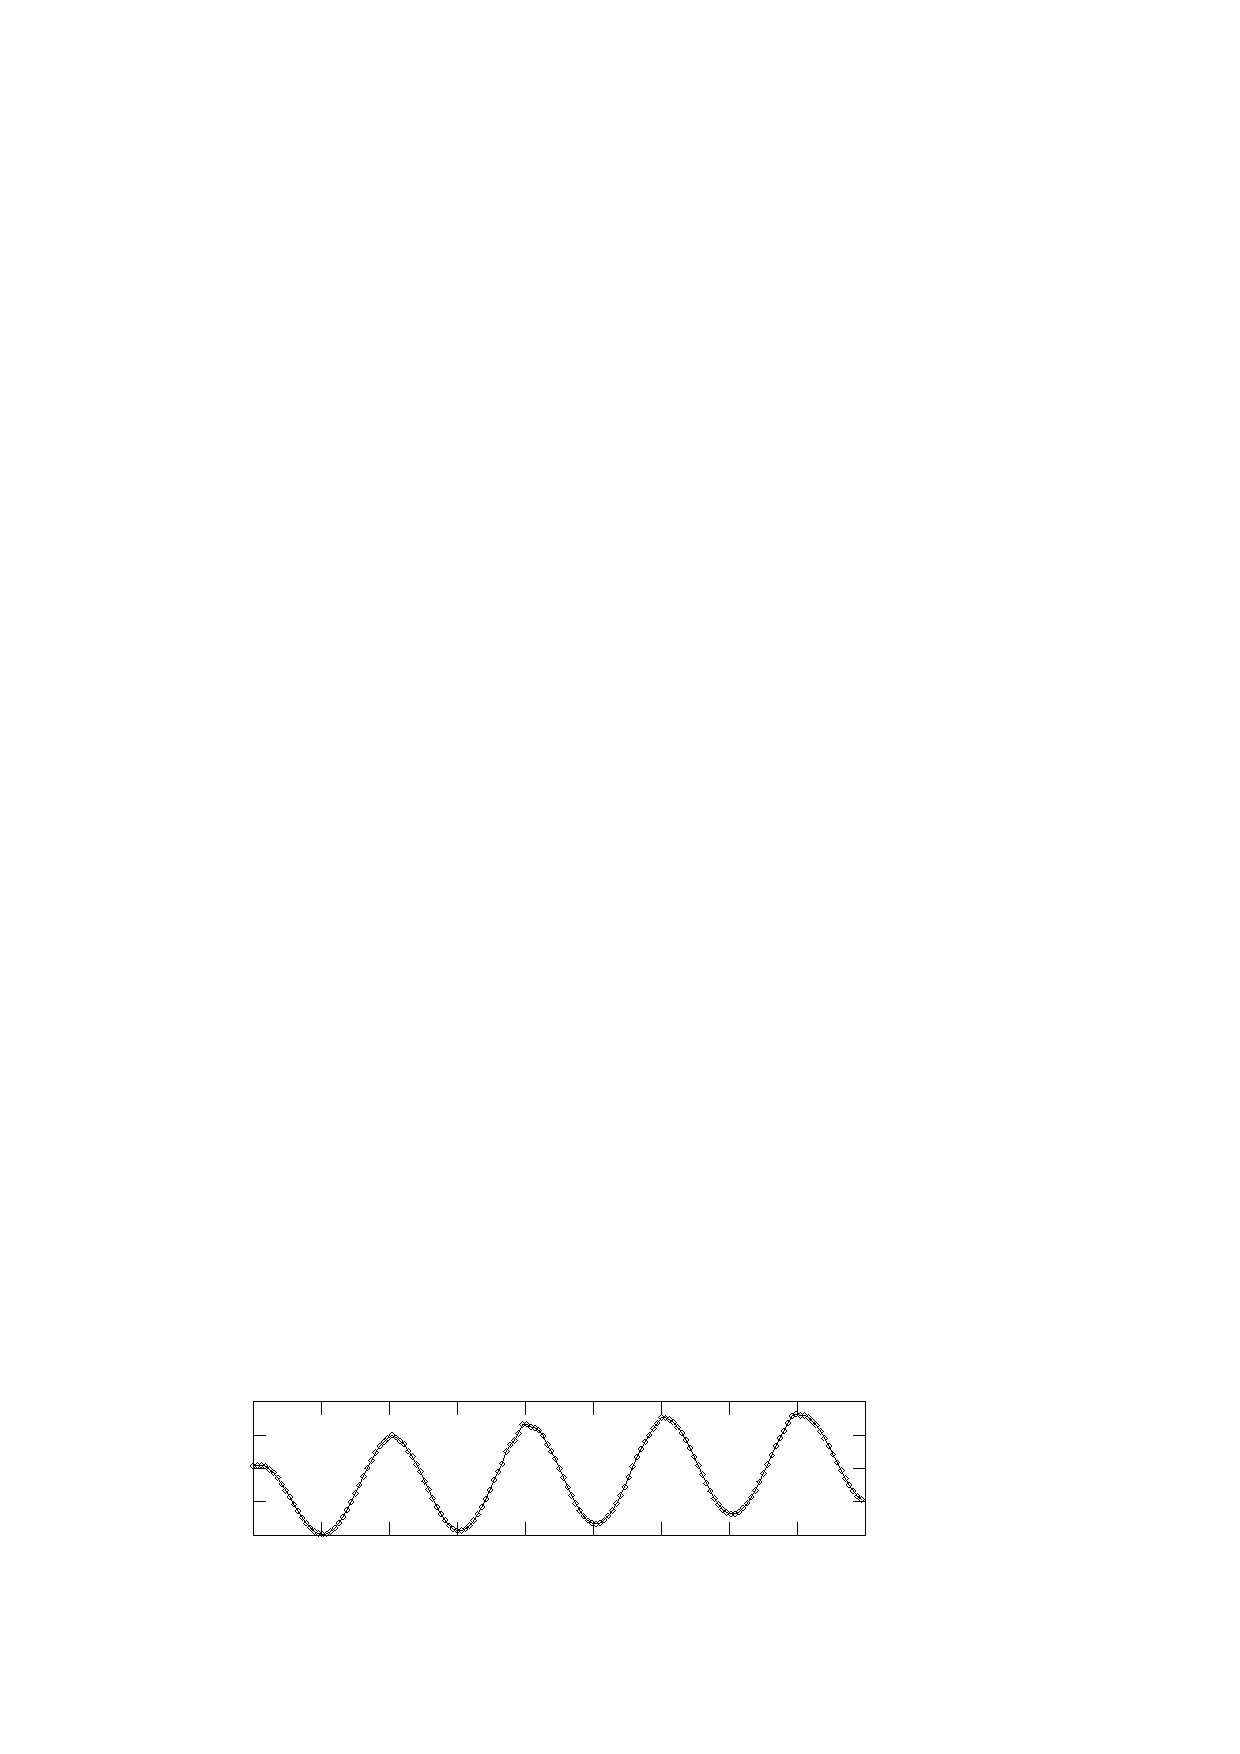
\includegraphics{eps/resonancia-cuadrada}%
\end{picture}%
\begingroup
\setlength{\unitlength}{0.0200bp}%
\begin{picture}(18000,5400)(0,0)%
\put(2200,1650){\makebox(0,0)[r]{\strut{} 0}}%
\put(2200,2450){\makebox(0,0)[r]{\strut{} 45}}%
\put(2200,3250){\makebox(0,0)[r]{\strut{} 90}}%
\put(2200,4050){\makebox(0,0)[r]{\strut{} 135}}%
\put(2200,4850){\makebox(0,0)[r]{\strut{} 180}}%
\put(2475,1100){\makebox(0,0){\strut{}0.25}}%
\put(4108,1100){\makebox(0,0){\strut{}0.50}}%
\put(5742,1100){\makebox(0,0){\strut{}0.75}}%
\put(7375,1100){\makebox(0,0){\strut{}1.00}}%
\put(9008,1100){\makebox(0,0){\strut{}1.25}}%
\put(10642,1100){\makebox(0,0){\strut{}1.50}}%
\put(12275,1100){\makebox(0,0){\strut{}1.75}}%
\put(13908,1100){\makebox(0,0){\strut{}2.00}}%
\put(15542,1100){\makebox(0,0){\strut{}2.25}}%
\put(17175,1100){\makebox(0,0){\strut{}2.50}}%
\put(550,3250){\rotatebox{90}{\makebox(0,0){\strut{}$P^\ast$}}}%
\put(9825,275){\makebox(0,0){\strut{}$h/\lambda$}}%
\end{picture}%
\endgroup
\endinput

\caption{\label{fig:resonancia-cuadrada}
Los picos en la potencia indican la ubicaci'on de lor primeros cinco modos resonantes para una cavidad cuadrada.
}
\end{figure}
La figura~\ref{fig:U-F} muestra el potencial  y la fuerza calculados con las ecuaciones 
derivadas por Gor'kov para una cavidad con un reflector plano en modo 5. De las
figuras (a) y (b) correspondientes al potencial y la fuerza, respectivamente, se puede
apreciar como en los m'inimos del potencial la fuerza es cero, lo que equivale a un
punto estable en un experimento en ausencia de gravedad. En un experimento bajo la
acci'on de un campo gravitatorio, las posiciones de levitaci'on de una part'icula de
radio $r$ seran aquellas donde el peso de esta sea igual a la fuerza generada por
el potencial ac'ustico. 


\begin{figure}
%GNUPLOT: LaTeX picture with Postscript
\begin{picture}(0,0)%
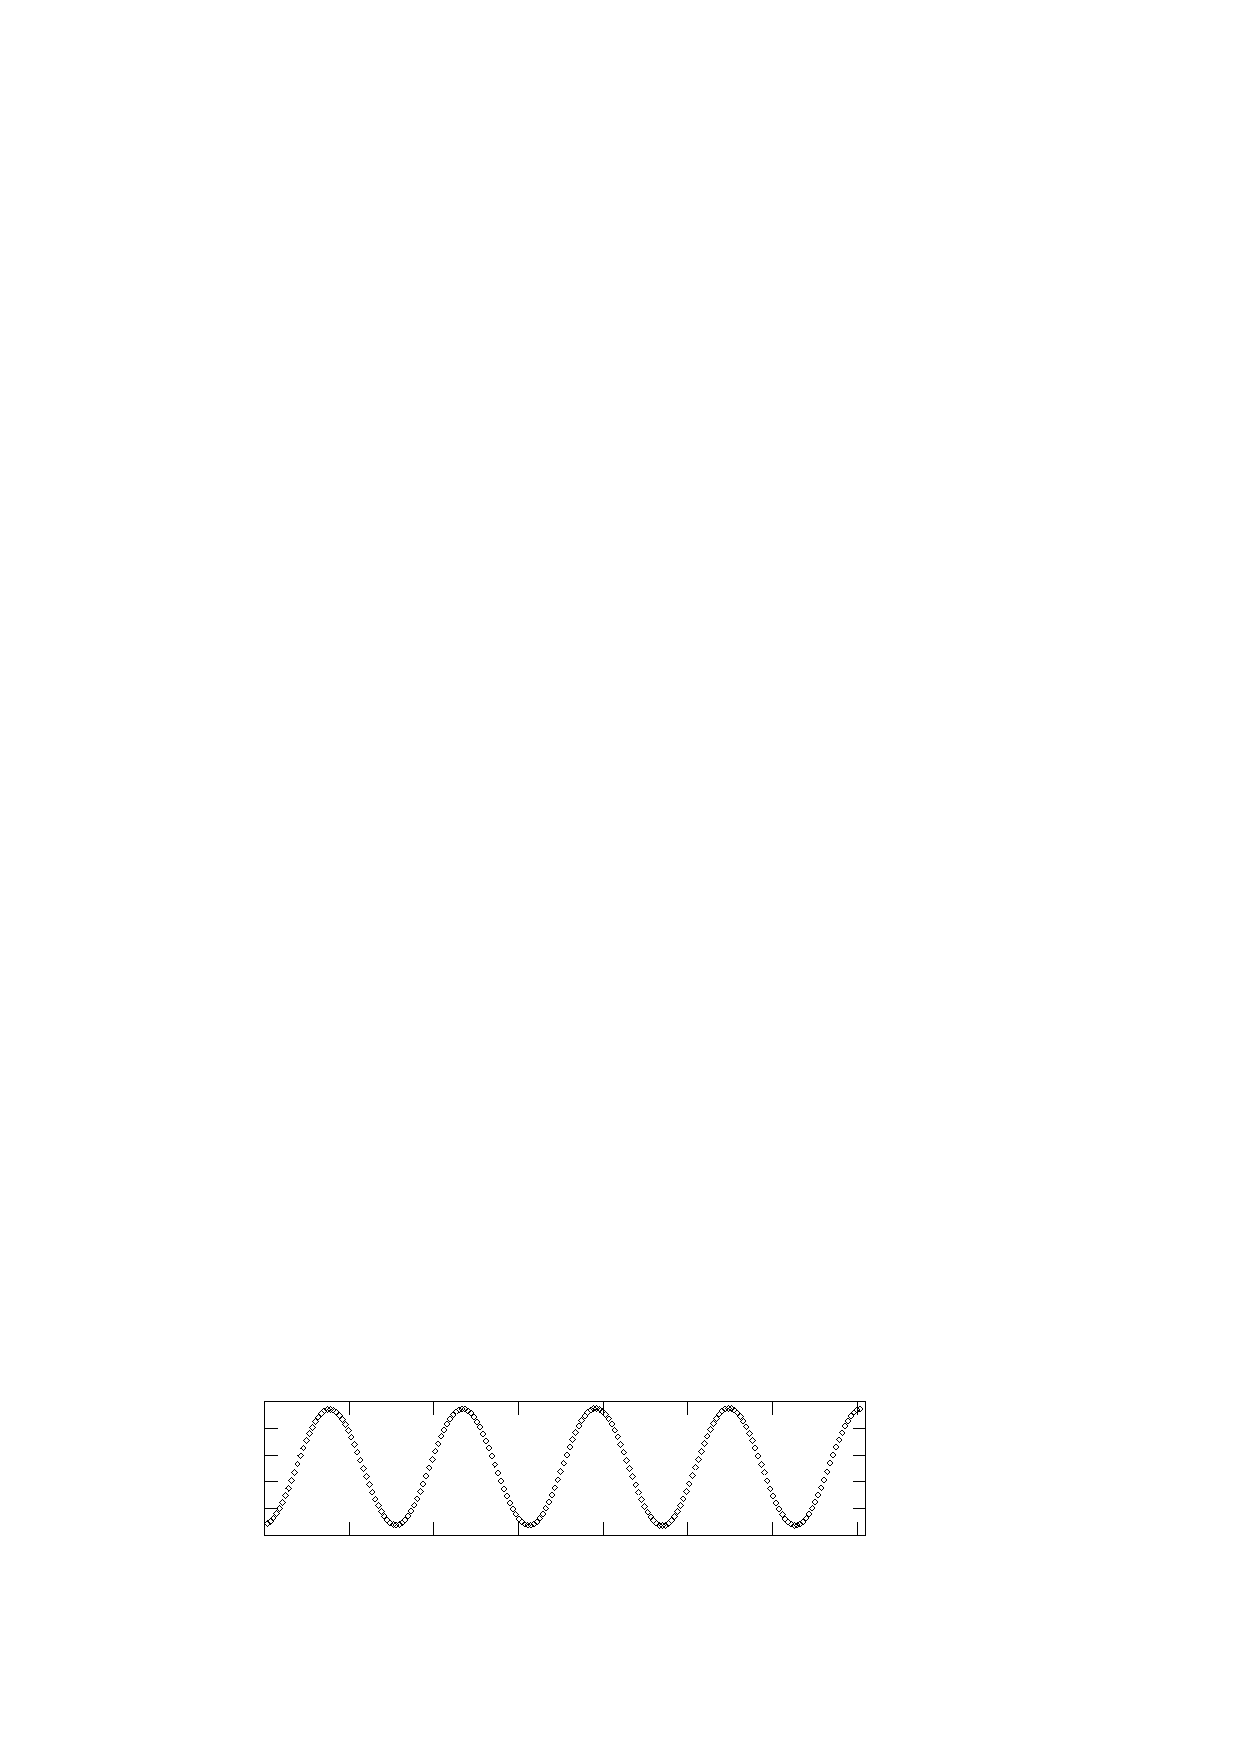
\includegraphics{eps/U}%
\end{picture}%
\begingroup
\setlength{\unitlength}{0.0200bp}%
\begin{picture}(18000,5400)(0,0)%
\put(2475,1650){\makebox(0,0)[r]{\strut{}-0.22}}%
\put(2475,2290){\makebox(0,0)[r]{\strut{}-0.15}}%
\put(2475,2930){\makebox(0,0)[r]{\strut{}-0.07}}%
\put(2475,3570){\makebox(0,0)[r]{\strut{}0.00}}%
\put(2475,4210){\makebox(0,0)[r]{\strut{}0.08}}%
\put(2475,4850){\makebox(0,0)[r]{\strut{}0.15}}%
\put(2750,1100){\makebox(0,0){\strut{} 0}}%
\put(4782,1100){\makebox(0,0){\strut{} 2}}%
\put(6813,1100){\makebox(0,0){\strut{} 4}}%
\put(8845,1100){\makebox(0,0){\strut{} 6}}%
\put(10877,1100){\makebox(0,0){\strut{} 8}}%
\put(12908,1100){\makebox(0,0){\strut{} 10}}%
\put(14940,1100){\makebox(0,0){\strut{} 12}}%
\put(16972,1100){\makebox(0,0){\strut{} 14}}%
\put(550,4550){\rotatebox{0}{\makebox(0,0){\strut{}(a)}}}%
\put(550,3250){\rotatebox{90}{\makebox(0,0){\strut{}$U^\ast$}}}%
\put(9962,275){\makebox(0,0){\strut{}$x^\ast$}}%
\end{picture}%
\endgroup
\endinput

%GNUPLOT: LaTeX picture with Postscript
\begin{picture}(0,0)%
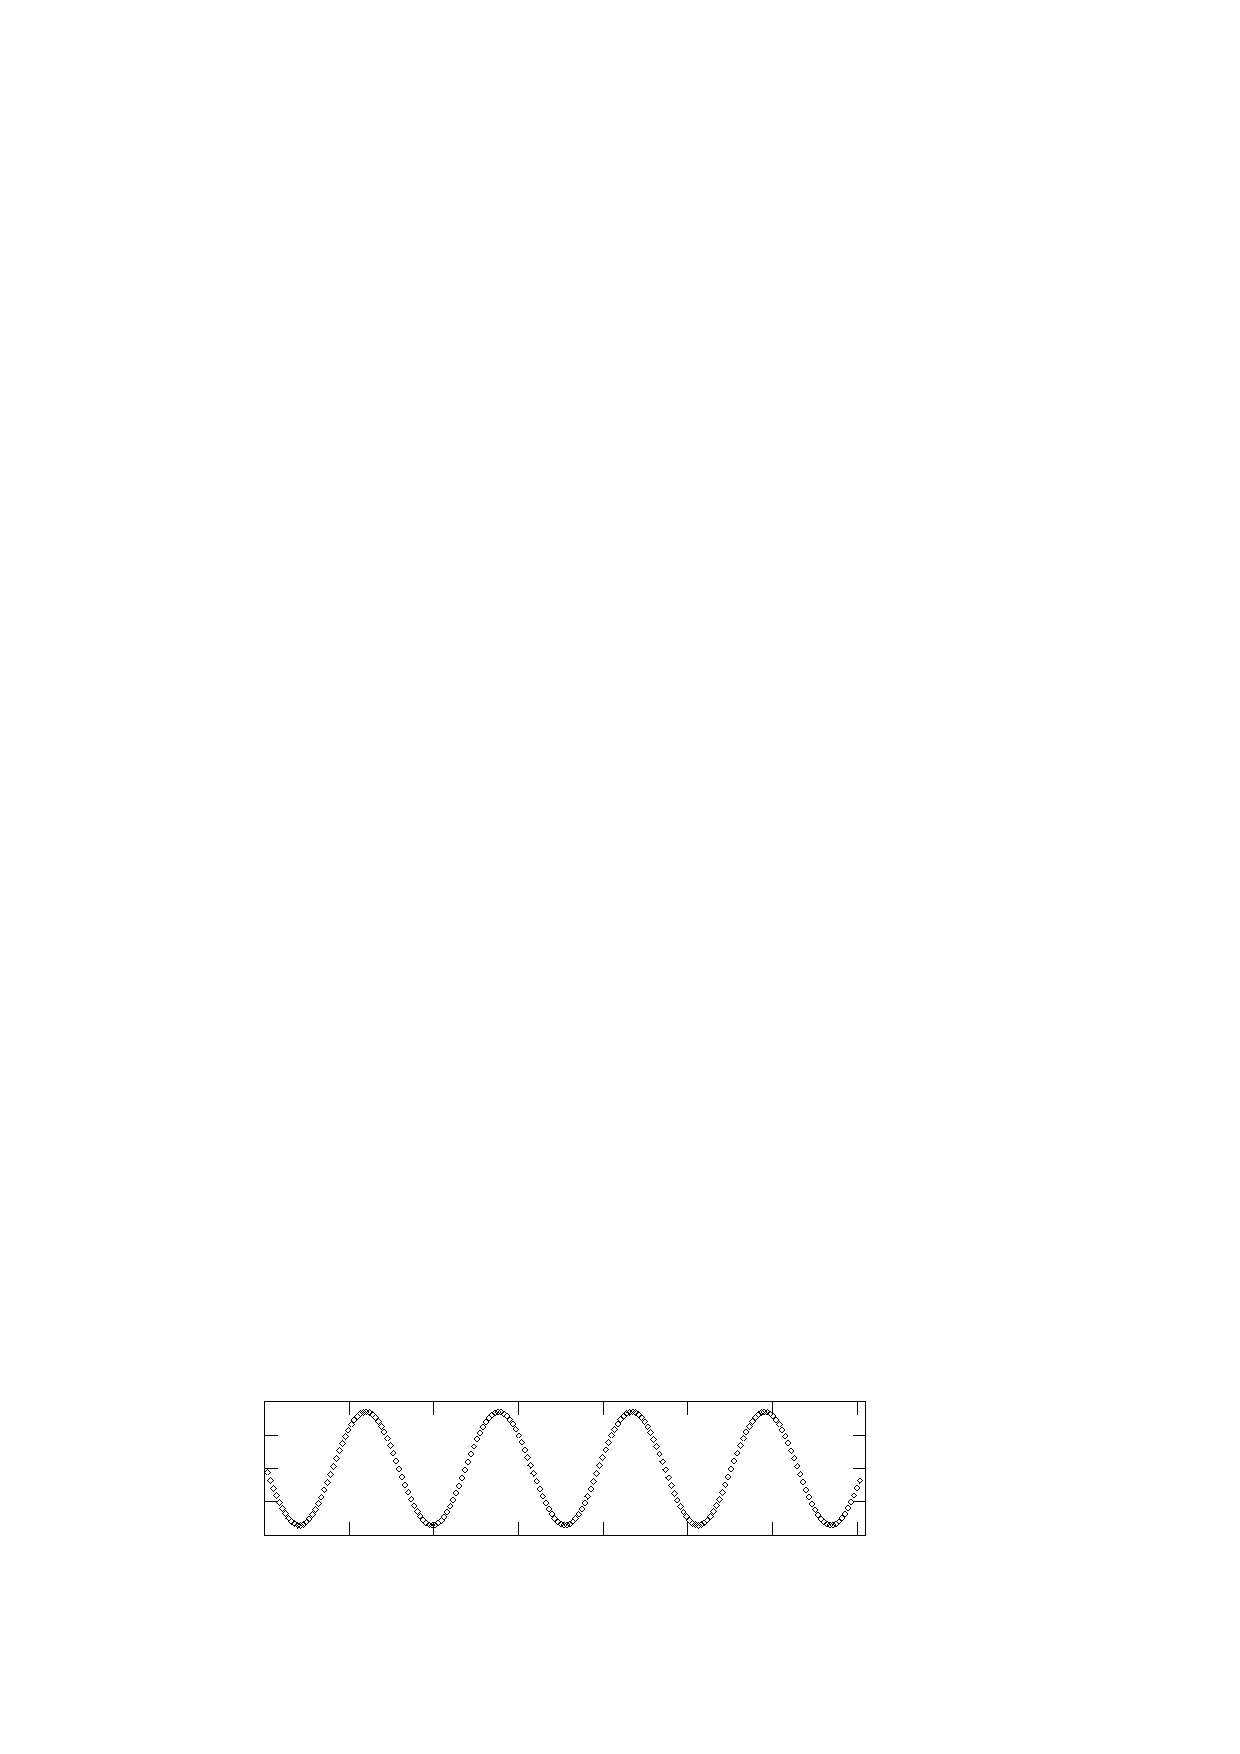
\includegraphics{eps/F}%
\end{picture}%
\begingroup
\setlength{\unitlength}{0.0200bp}%
\begin{picture}(18000,5400)(0,0)%
\put(2475,1650){\makebox(0,0)[r]{\strut{}-0.50}}%
\put(2475,2450){\makebox(0,0)[r]{\strut{}-0.25}}%
\put(2475,3250){\makebox(0,0)[r]{\strut{}0.00}}%
\put(2475,4050){\makebox(0,0)[r]{\strut{}0.25}}%
\put(2475,4850){\makebox(0,0)[r]{\strut{}0.50}}%
\put(2750,1100){\makebox(0,0){\strut{} 0}}%
\put(4782,1100){\makebox(0,0){\strut{} 2}}%
\put(6813,1100){\makebox(0,0){\strut{} 4}}%
\put(8845,1100){\makebox(0,0){\strut{} 6}}%
\put(10877,1100){\makebox(0,0){\strut{} 8}}%
\put(12908,1100){\makebox(0,0){\strut{} 10}}%
\put(14940,1100){\makebox(0,0){\strut{} 12}}%
\put(16972,1100){\makebox(0,0){\strut{} 14}}%
\put(550,4550){\rotatebox{0}{\makebox(0,0){\strut{}(b)}}}%
\put(550,3250){\rotatebox{90}{\makebox(0,0){\strut{}$F^\ast$}}}%
\put(9962,275){\makebox(0,0){\strut{}$x^\ast$}}%
\end{picture}%
\endgroup
\endinput

\caption{\label{fig:U-F}
(a) Potencial ac'ustico para una cavidad con $L_y^\ast=14.1$ correspondiente al modo 5.
(b) Fuerza ac'ustica a lo alto de la cavidad.
}
\end{figure}
En la figura~\ref{fig:F-wp} se muestran la fuerza ac'ustica calculada a partir del
potencial y la l'inea continua representa a una part'icula s'olida de peso $w_p^\ast=0.25$.
Las intersecciones con la fuerza indican las posiciones donde ambas fuerzas se equilibran.
De esta figura, correspondiente al modo 5, se observan 8 puntos de intersecci'on, de
estos, lo que se encuentran cerca del pozo del potencial, son los puntos estables, y el
resto son puntos inestables. Los puntos estables, act'uan como un atractor y las particulas
se acercan a ellos flotando o cayendo, dependiendo de la posici'on inicial en que se coloquen,
como se muestra en la figura[aqu'i va la figura de las trayectorias]. En esta figura, se
muestran la trayectoria de particulas de radio $r^\ast=0.927$ al ser colocadas en diferentes
posiciones iniciales.
\begin{figure}
%GNUPLOT: LaTeX picture with Postscript
\begin{picture}(0,0)%
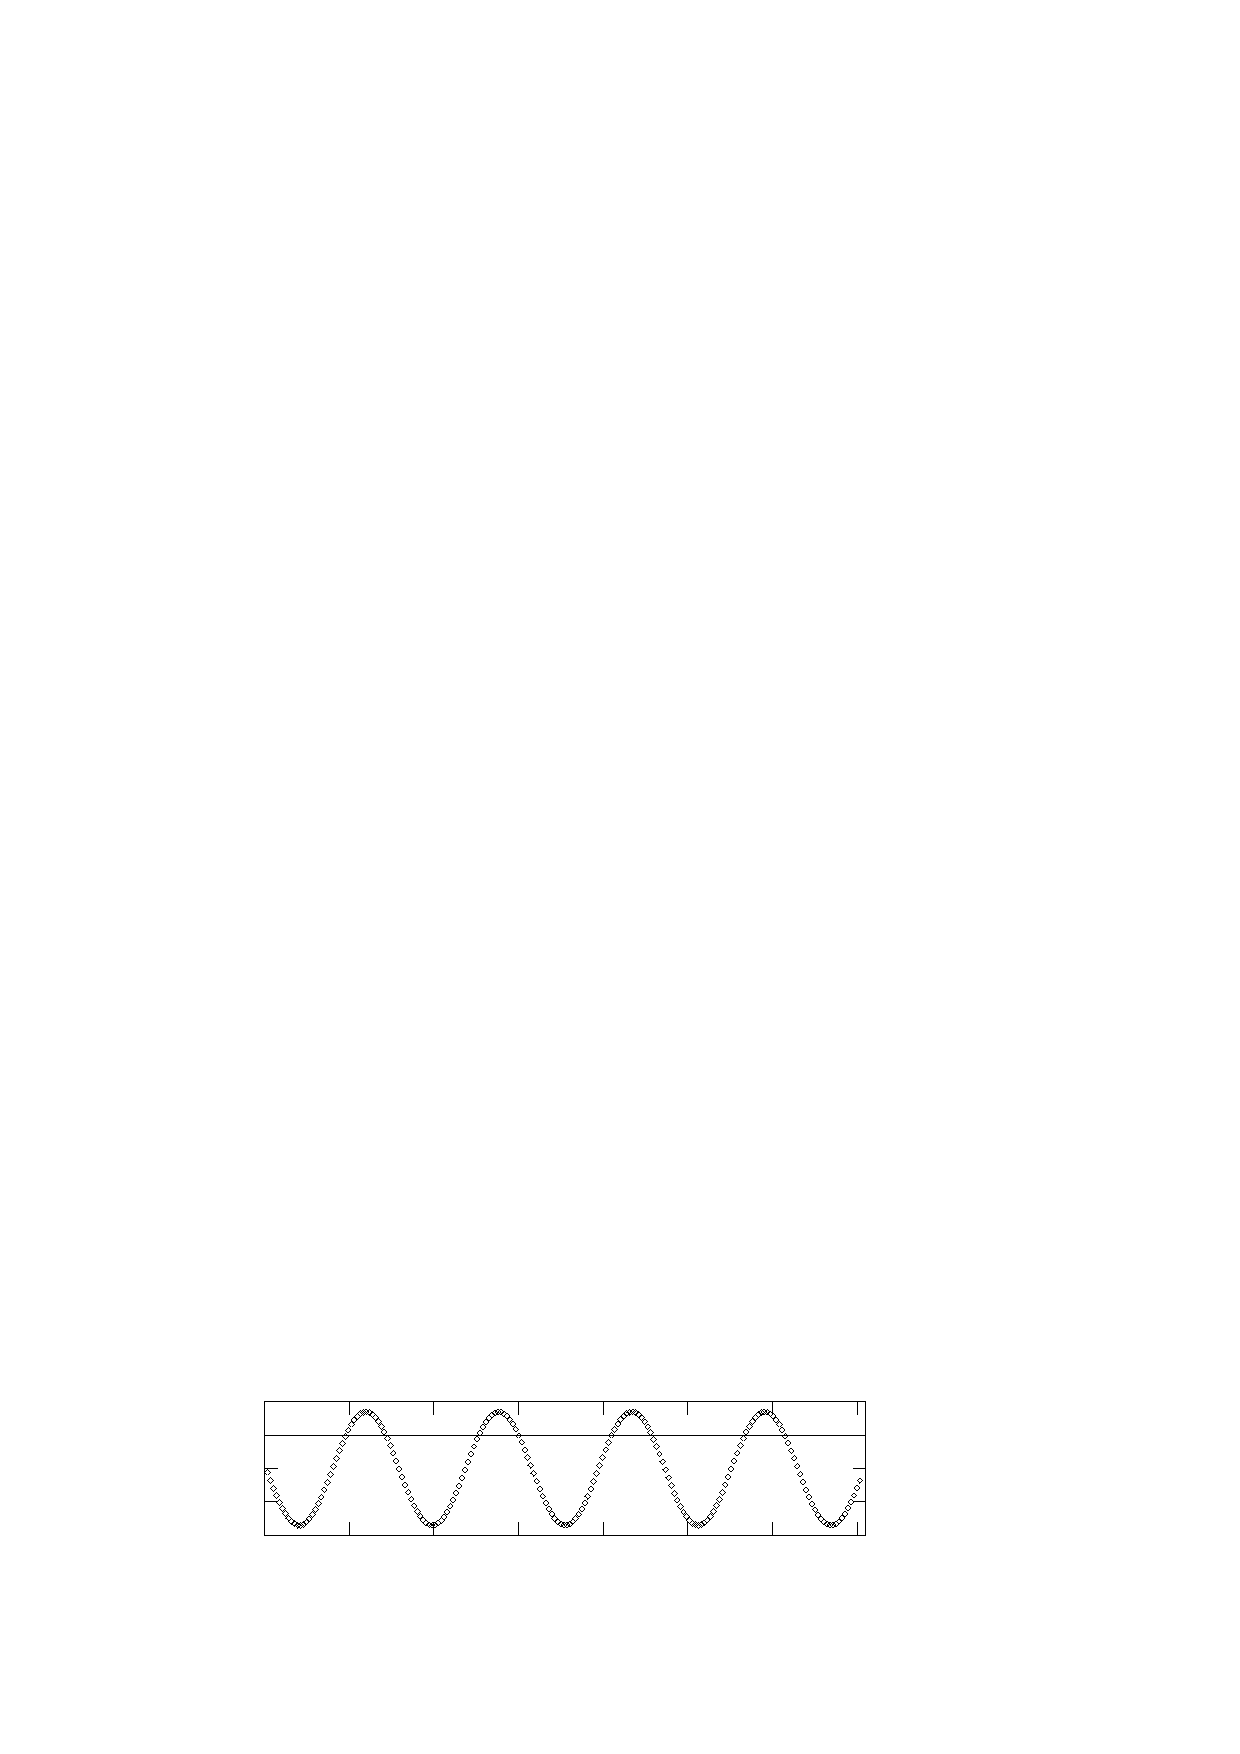
\includegraphics{eps/F-wp}%
\end{picture}%
\begingroup
\setlength{\unitlength}{0.0200bp}%
\begin{picture}(18000,5400)(0,0)%
\put(2475,1650){\makebox(0,0)[r]{\strut{}-0.50}}%
\put(2475,2450){\makebox(0,0)[r]{\strut{}-0.25}}%
\put(2475,3250){\makebox(0,0)[r]{\strut{}0.00}}%
\put(2475,4050){\makebox(0,0)[r]{\strut{}0.25}}%
\put(2475,4850){\makebox(0,0)[r]{\strut{}0.50}}%
\put(2750,1100){\makebox(0,0){\strut{} 0}}%
\put(4782,1100){\makebox(0,0){\strut{} 2}}%
\put(6813,1100){\makebox(0,0){\strut{} 4}}%
\put(8845,1100){\makebox(0,0){\strut{} 6}}%
\put(10877,1100){\makebox(0,0){\strut{} 8}}%
\put(12908,1100){\makebox(0,0){\strut{} 10}}%
\put(14940,1100){\makebox(0,0){\strut{} 12}}%
\put(16972,1100){\makebox(0,0){\strut{} 14}}%
\put(550,3250){\rotatebox{90}{\makebox(0,0){\strut{}$F^\ast$}}}%
\put(9962,275){\makebox(0,0){\strut{}$x^\ast$}}%
\end{picture}%
\endgroup
\endinput

\caption{\label{fig:F-wp}
Fuerza debida al potencial a lo alto de la cavidad. La l'inea continua
representa el peso de la part'icula y las intersecciones marcan la altura
donde la fuerza es igual al peso de la part'icula.
}
\end{figure}
Justificar el porque del cambio de geometr'ia, y 
describir el dispositivo y las condiciones de frontera.

Encontrar las frecuencias donde hay resonancia, con la gr'afica
de Xie de potencia vs frecuencia.

Una vez encontrada la frecuencia de resonancia hacer 
experimentos y mostrar que se puede levitar una particula
m'as pesada con la misma fuerza aplicada en el piezoelectrico.
Mostrar potencial.

Dejar las particulas en varias posiciones y rastrear su trajectoria,
mostrar campos de velocidades y explicarlos un poco.
Flujo alrededor de la part'icula.


